% This is a Basic Assignment Paper but with like Code and stuff allowed in it. 

\documentclass[11pt]{article}

% Preamble

\usepackage[margin=1in]{geometry}
\usepackage{amsfonts, amsmath, amssymb}
\usepackage{fancyhdr, float, graphicx}
\usepackage[utf8]{inputenc} % Required for inputting international characters
\usepackage[T1]{fontenc} % Output font encoding for international characters
\usepackage{fouriernc} % Use the New Century Schoolbook font
\usepackage[nottoc, notlot, notlof]{tocbibind}
\usepackage{listings}
\usepackage{xcolor}
\usepackage{float}

\definecolor{codegreen}{rgb}{0,0.6,0}
\definecolor{codegray}{rgb}{0.5,0.5,0.5}
\definecolor{codepurple}{rgb}{0.58,0,0.82}
\definecolor{backcolour}{rgb}{0.95,0.95,0.92}

\lstdefinestyle{mystyle}{
    backgroundcolor=\color{backcolour},   
    commentstyle=\color{codegreen},
    keywordstyle=\color{magenta},
    numberstyle=\tiny\color{codegray},
    stringstyle=\color{codepurple},
    basicstyle=\ttfamily\footnotesize,
    breakatwhitespace=false,         
    breaklines=true,                 
    captionpos=b,                    
    keepspaces=true,                 
    numbers=left,                    
    numbersep=5pt,                  
    showspaces=false,                
    showstringspaces=false,
    showtabs=false,                  
    tabsize=2
}

\lstset{style=mystyle}

% Header and Footer
\pagestyle{fancy}
\fancyhead{}
\fancyfoot{}
\fancyhead[L]{\textit{\Large{Computer Networks Assignment 1}}}
%\fancyhead[R]{\textit{something}}
\fancyfoot[C]{\thepage}
\renewcommand{\footrulewidth}{1pt}



% Other Doc Editing
% \parindent 0ex
%\renewcommand{\baselinestretch}{1.5}

\begin{document}
	
	\begin{titlepage} 
		\centering 
		
		%---------------------------NAMES-------------------------------
		
		\huge\textsc{
			MIT World Peace University
		}\\
	
		\vspace{0.75\baselineskip} % space after Uni Name
		
		\LARGE{
			Computer Networks\\
			Second Year B. Tech, Semester 3
		}
		
		\vfill % space after Sub Name
		
		%--------------------------TITLE-------------------------------
		
		\rule{\textwidth}{1.6pt}\vspace*{-\baselineskip}\vspace*{2pt}
		\rule{\textwidth}{0.6pt}
		\vspace{0.75\baselineskip} % Whitespace above the title
		
		
		
		\huge{\textsc{
			Configuration of a Simple LAN
			}} \\
		
		
		
		\vspace{0.5\baselineskip} % Whitespace below the title
		\rule{\textwidth}{0.6pt}\vspace*{-\baselineskip}\vspace*{2.8pt}
		\rule{\textwidth}{1.6pt}
		
		\vspace{1\baselineskip} % Whitespace after the title block

		%--------------------------SUBTITLE --------------------------	
			
		\LARGE\textsc{
			Practical Report
		} % Subtitle or further description
		\vfill
		
		%--------------------------AUTHOR-------------------------------
		
		Prepared By
		\vspace{0.5\baselineskip} % Whitespace before the editors
		
		\Large{
			Krishnaraj Thadesar \\
			Cyber Security and Forensics\\
			Batch A2, PA 34
		}
		
		
		\vspace{0.5\baselineskip} % Whitespace below the editor list
		\today

	\end{titlepage}
	
	
\tableofcontents
\thispagestyle{empty}
\clearpage


\setcounter{page}{1}

\section{Aim and Objectives}
To learn how to configure a simple LAN connection using Cisco Packet Tracer.

\section{Devices}

\subsection{Devices Used}
\begin{enumerate}
	\item 1 Generic Switch
	\item 2 Switch 2960 with 24 LAN Ports
	\item 6 Generic PCs
	\item 4 Laptops
\end{enumerate}

\subsection{Device Info and IP Addresses}

Subnet Mask: 255.255.255.0

\begin{table}[H] 
	\centering
	\begin{tabular}{|c|c|c|}
	\hline
	\textbf{Name} & \textbf{Type}      & \textbf{IP}    \\ 
	\hline
	PC0           & PC                 & 192.168.10.1   \\ 
	\hline
	PC1           & PC                 & 192.168.10.2   \\ 
	\hline
	PC2           & PC                 & 192.168.10.3   \\ 
	\hline
	PC3           & PC                 & 192.168.10.4   \\ 
	\hline
	PC4           & PC                 & 192.168.10.5   \\ 
	\hline
	PC5           & PC                 & 192.168.10.6   \\ 
	\hline
	Laptop0       & Laptop             & 192.168.10.7   \\ 
	\hline
	Laptop1       & Laptop             & 192.168.10.8   \\ 
	\hline
	Laptop2       & Laptop             & 192.168.10.9   \\ 
	\hline
	Laptop3       & Laptop             & 192.168.10.10  \\ 
	\hline
	Switch0       & 2950-24
					Switch & None           \\ 
	\hline
	Switch1       & 2950-24
					Switch & None           \\ 
	\hline
	Switch2       & Generic
					Switch & None           \\
	\hline
	\end{tabular}
	\end{table}

\section{Cables}
\begin{enumerate}
	\item Straight LAN Cable to connect unlike Devices
	\item Crossover LAN Cable to connect like Devices
\end{enumerate}

\section{Procedure to Configure LAN}
\begin{enumerate}
	\item All 3 switches are connected with each other using crossover cables, as they are similar. 
	\item 4 PCs are connected to The first Switch
    \item 4 Laptops are connected to the Second switch
    \item 2 More computers are connected to another Switch. 
    \item Check the connection by opening the command prompt, and entering the commands ipconfig, and pinging the other computers. 
\end{enumerate}

\section{Commands}

\begin{enumerate}
	\item \textbf{ipconfig}: 
	
	In Windows, ipconfig is a console application designed to run from the Windows command prompt. This utility allows you to get the IP address information of a Windows computer. It also allows some control over your network adapters, IP addresses (DHCP-assigned specifically), even your DNS cache. Ipconfig replaced the older winipcfg utility.
	\item \textbf{ping <ip addr>}: 
	
	The ping command is a Command Prompt command used to test the ability of the source computer to reach a specified destination computer. It's a simple way to verify that a computer can communicate with another computer or network device.\\ 
	The ping command operates by sending Internet Control Message Protocol (ICMP) Echo Request messages to the destination computer and waiting for a response. The two major pieces of information that the ping command provides are how many of those responses are returned and how long it takes for them to return.
\end{enumerate}

\section{Platform}
	\textbf{Operating System}: Arch Linux x86-64\\
	\textbf{IDEs or Text Editors Used}: Visual Studio Code\\
	\textbf{Programs Used}: Cisco Packet Tracer v6.0.1

\section{Output}

\begin{lstlisting}
FastEthernet0 Connection:(default port)

Link-local IPv6 Address.........: FE80::201:C9FF:FEE6:3985
IP Address......................: 192.168.1.1
Subnet Mask.....................: 255.255.255.0
Default Gateway.................: 0.0.0.0

PC>ping 192.168.1.2

Pinging 192.168.1.2 with 32 bytes of data:

Reply from 192.168.1.2: bytes=32 time=1ms TTL=128
Reply from 192.168.1.2: bytes=32 time=17ms TTL=128
Reply from 192.168.1.2: bytes=32 time=0ms TTL=128
Reply from 192.168.1.2: bytes=32 time=0ms TTL=128

Ping statistics for 192.168.1.2:
Packets: Sent = 4, Received = 4, Lost = 0 (0% loss),
Approximate round trip times in milli-seconds:
Minimum = 0ms, Maximum = 17ms, Average = 4ms

\end{lstlisting}

\section{Connection Screenshot}


\begin{figure}[H]
	\centering
	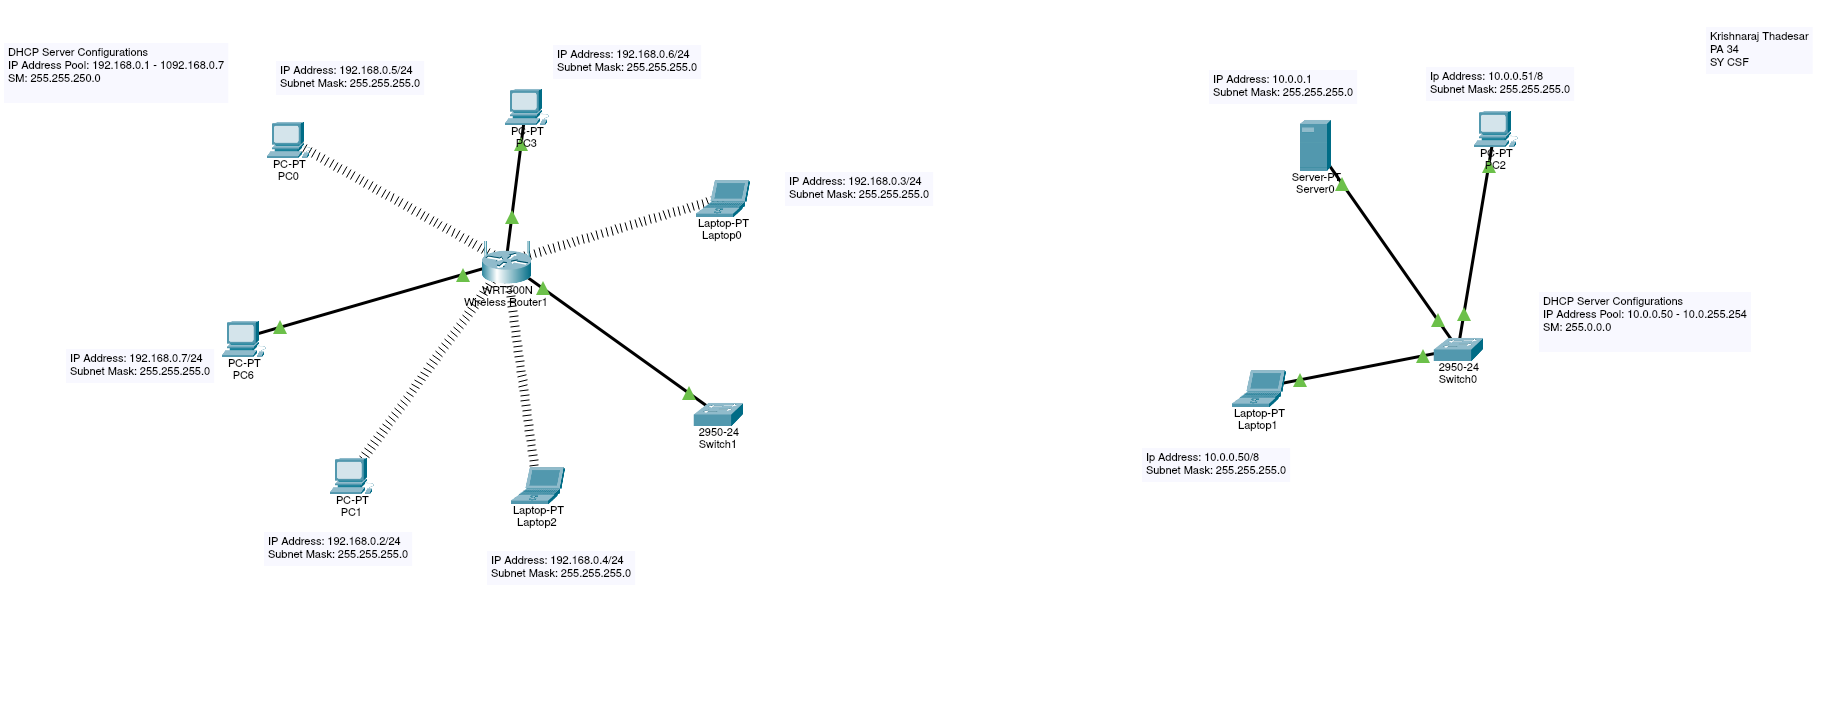
\includegraphics[scale=0.47]{Screenshots/Assignment_2_screenshot.png}
\end{figure}


\section{Conclusion}
A local area network was successfully created, deployed and tested on a simulator. The concept behind the Local area network was understood in detail. The various types of cables used to connect the devices were also used and explained. Commands to test computers on a network were also executed successfully. Various computers can be connected with each other and communicate seamlessly with the help of switches, Network Interface Cards, Computers and Straight as well as twisted Ethernet Cables.  in a local area network. 

\end{document}